\documentclass{beamer}

\usetheme[pageofpages=of,% String used between the current page and the
                         % total page count.
          bullet=circle,% Use circles instead of squares for bullets.
          titleline=true,% Show a line below the frame title.
          alternativetitlepage=true,% Use the fancy title page.
          titlepagelogo=celery-logo,% Logo for the first page.
          watermark=celery-logo,% Watermark used in every page.
          watermarkheight=25px,% Height of the watermark.
          watermarkheightmult=20,% The watermark image is 4 times bigger
                                % than watermarkheight.
          ]{Torino}


\title{Celery - Distributed Task Queue}
\author{Mike DeLaurentis}
\date{May 21, 2013}

\begin{document}

\begin{frame}[plain]
\titlepage
\end{frame}

\begin{frame}
  \frametitle{What is it?}
  \begin{itemize}
  \item Distributed task queue
  \item Can run tasks in one process,
  \item ... or mulitple processes on one machine
  \item ... or multiple machines
  \end{itemize}
\end{frame}

\begin{frame}
  \frametitle{Setting up}
  \begin{columns}
    \begin{column}{0.5\textwidth}
      \begin{itemize}
      \item Installs easily with pip
      \item Needs a ``broker'' (like RabbitMQ, Redis, or relational DB) to hold tasks
      \item May need a ``backend'' if you want direct access to results
      \item Config is easy,
      \item either with a simple file
      \item or programmatically
      \end{itemize}      
    \end{column}

    \begin{column}{0.5\textwidth}

      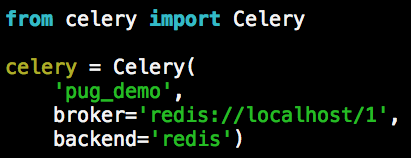
\includegraphics[scale=0.4]{config.png}

    \end{column}
  \end{columns}
\end{frame}

\begin{frame}
  \frametitle{Writing tasks}

  \begin{columns}
    \begin{column}{0.4\textwidth}

  \begin{itemize}
  \item Define tasks as decorated functions
  \item Takes serializable args
  \item Can return some result
  \item ... or store it elsewhere
  \end{itemize}
  \end{column}
    \begin{column}{0.6\textwidth}
      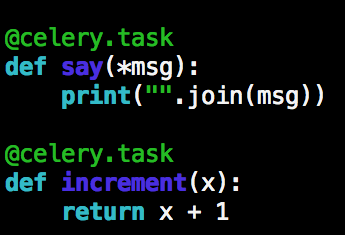
\includegraphics[scale=0.4]{tasks.png}
    \end{column}
  \end{columns}
\end{frame}

\begin{frame}
  \frametitle{Running workers}
  \begin{itemize}
  \item Start a worker by running 'celery' 
  \item Identify module with tasks using {\tt --app}
  \item Specify number of threads with {\tt --concurrency}
  \end{itemize}
  \begin{center}
    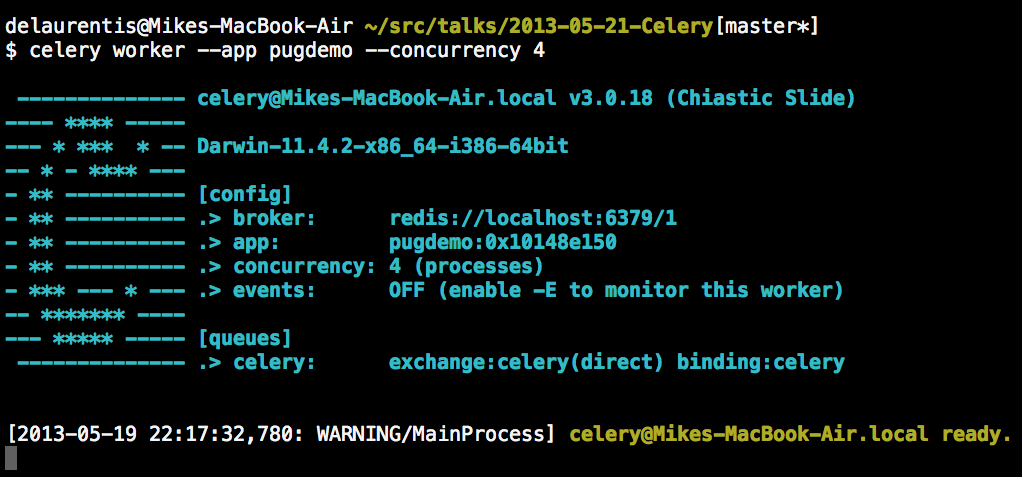
\includegraphics[scale=0.3]{startworker.png}    
  \end{center}
\end{frame}

\begin{frame}
  \frametitle{Submitting tasks}
  \begin{columns}
    \begin{column}{0.55\textwidth}

      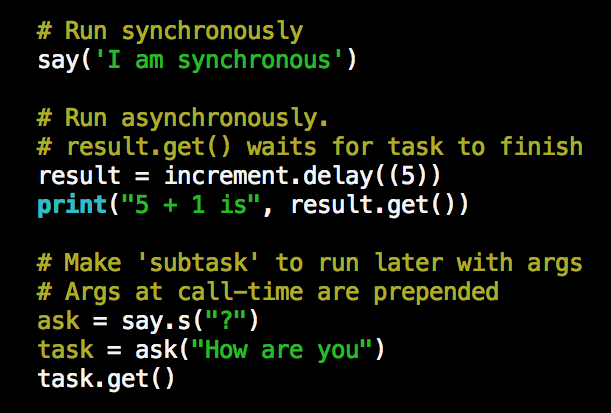
\includegraphics[scale=0.3]{runtasks.png}

    \end{column}
    \begin{column}{0.45\textwidth}
      \begin{itemize}
      \item Calling directly will run in process
      \item Call {\tt delay(*args)} to put on queue
      \item Call {\tt s(*args)} to make task object
      \end{itemize}
    \end{column}
  \end{columns}
\end{frame}


\begin{frame}
  \frametitle{Creating workflows}
  \begin{Large}
  \begin{itemize}
  \item Build a workflow programatically, out of:
    \begin{itemize}
  \item chain - List of tasks that must be run in order
  \item group - Tasks that can be run simultaneously
  \item chord - Group with callback
  \item chunks - Split a task with a long list of args into smaller tasks
    \end{itemize}
    \item Compose these elements to make complex workflows
  \end{itemize}
    
  \end{Large}

\end{frame}

\begin{frame}
  \frametitle{Immutable workflow}
  \begin{center}
  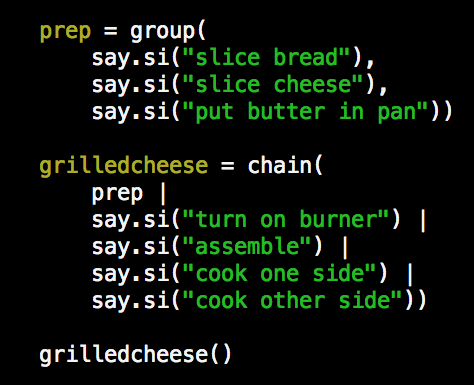
\includegraphics[scale=0.4]{wf1.png}
  \end{center}
\end{frame}

\begin{frame}
  \frametitle{Mutable workflow}
  \begin{center}
  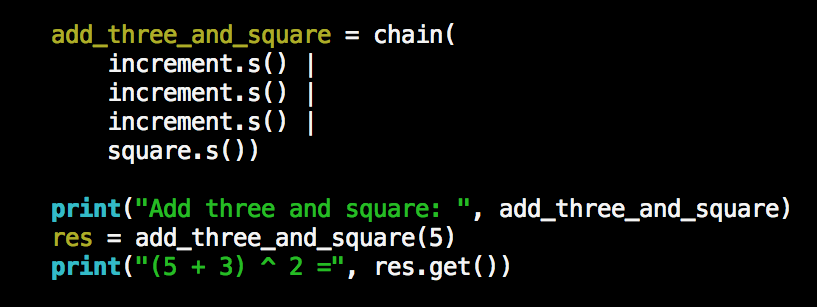
\includegraphics[scale=0.35]{wf2.png}
    
  \end{center}
\end{frame}

\begin{frame}
  \begin{LARGE}
    \begin{center}
      Thanks!
    \end{center}
  \end{LARGE}
\end{frame}

\end{document}

% 22,000
% 22,000,000
